\chapter{Adding Virtual Machine Images}
%Intro\footnotemark\\
\begin{spacing}{1.2}
%note en bas de page
\section{KVM installation }

\par Kernel-based Virtual Machine is a virtualization module in the Linux kernel that allows the
kernel to function as a hypervisor. So for the installation, we can do it like
indicated below : 
\\
\begin{figure}[!htb] 
\begin{center} 
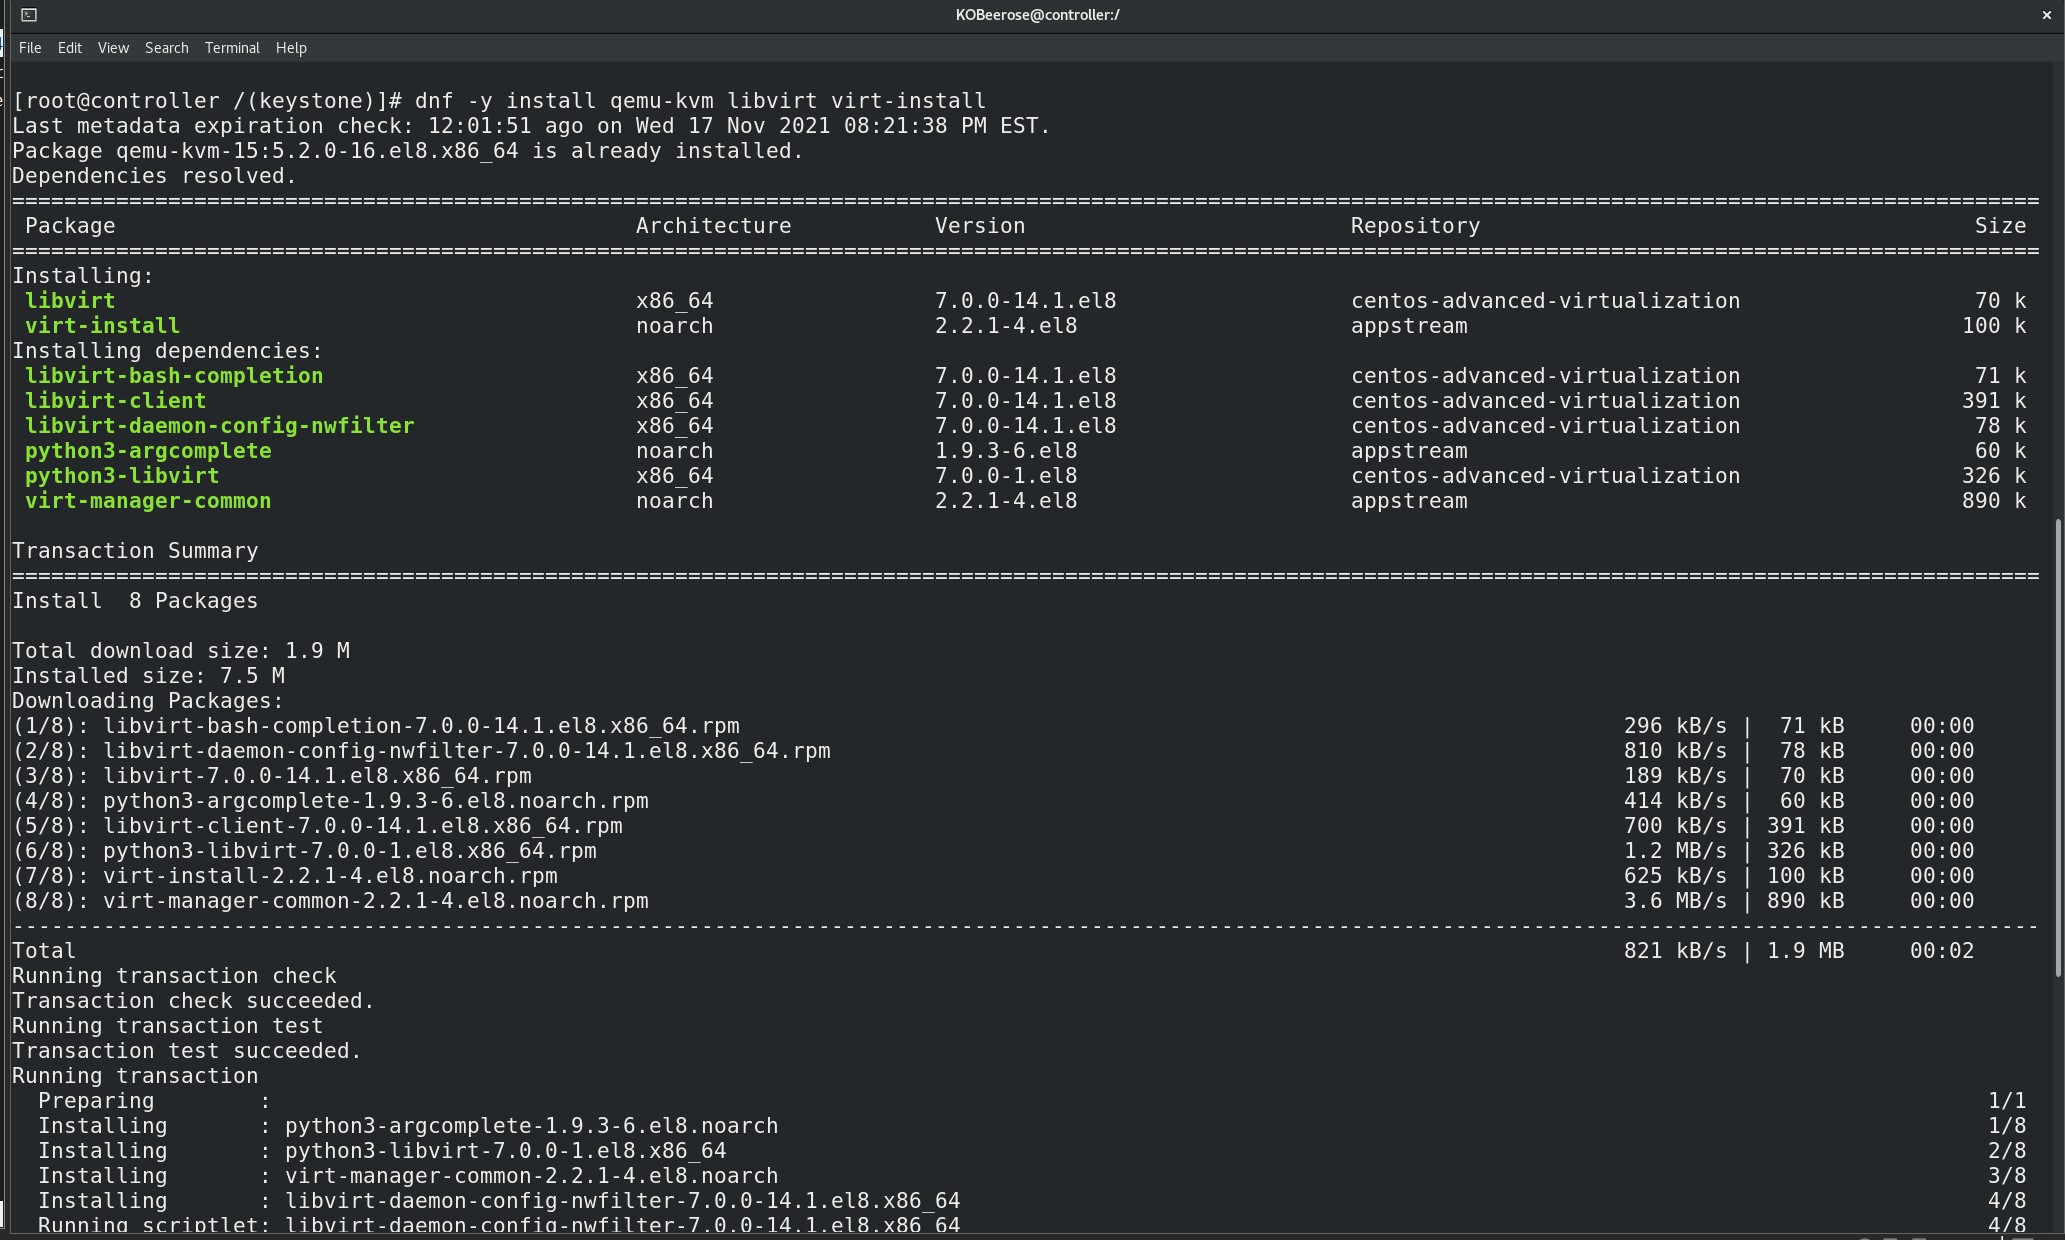
\includegraphics[width=1\linewidth]{Cloud/Add Virtual Machine Images/KVM Install/Installing qemu-kvm libvirt} 
\end{center} 
\caption{Installing qemu-kvm libvirt} 
\end{figure}  \FloatBarrier
\\

\par After the installation, we will confirm that the modules are loaded, and activate libvirtd. 
\\
\begin{figure}[!htb] 
\begin{center} 
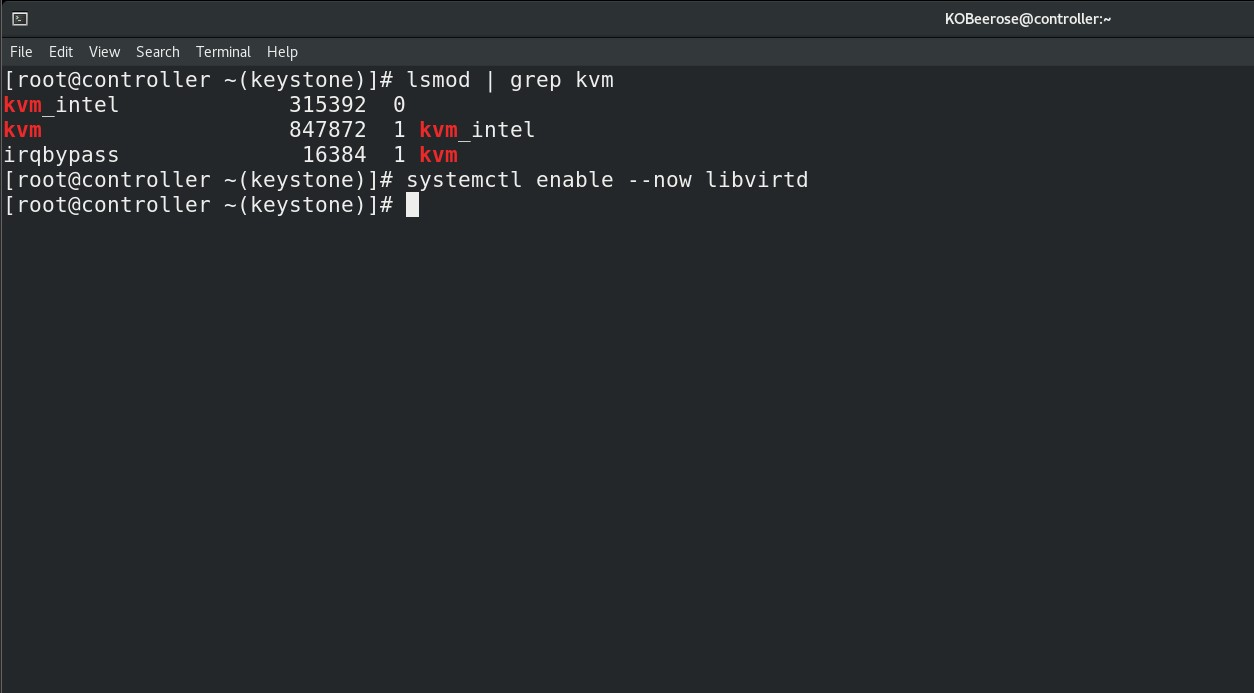
\includegraphics[width=1\linewidth]{Cloud/Add Virtual Machine Images/KVM Install/Enabling libvirtd} 
\end{center} 
\caption{Enabling libvirtd} 
\end{figure}  \FloatBarrier
\\

\par now we Configure Bridge networking for KVM virtual machines. Then we remove the network interface "ens37" and add it again as a member of "br0"
\\
\begin{figure}[!htb] 
\begin{center} 
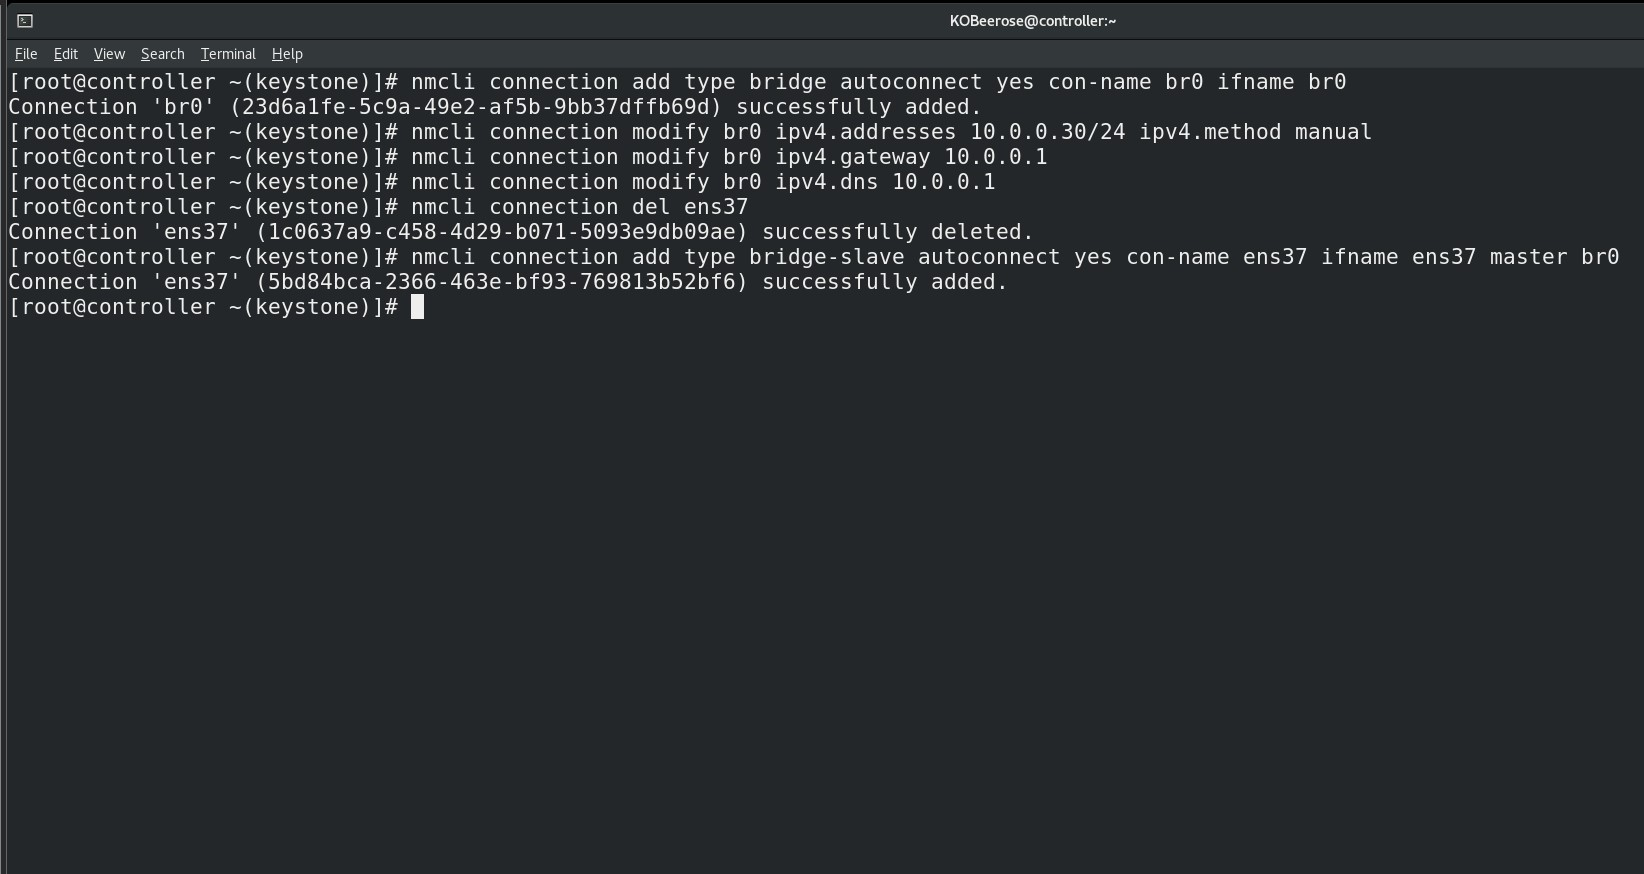
\includegraphics[width=1\linewidth]{Cloud/Add Virtual Machine Images/KVM Install/Configuring Bridge Net for KVM} 
\end{center} 
\caption{Configuring Bridge Net for KVM} 
\end{figure}  \FloatBarrier
\\

\par we make sure that the network interfaces are configured as we want.
\\
\begin{figure}[!htb] 
\begin{center} 
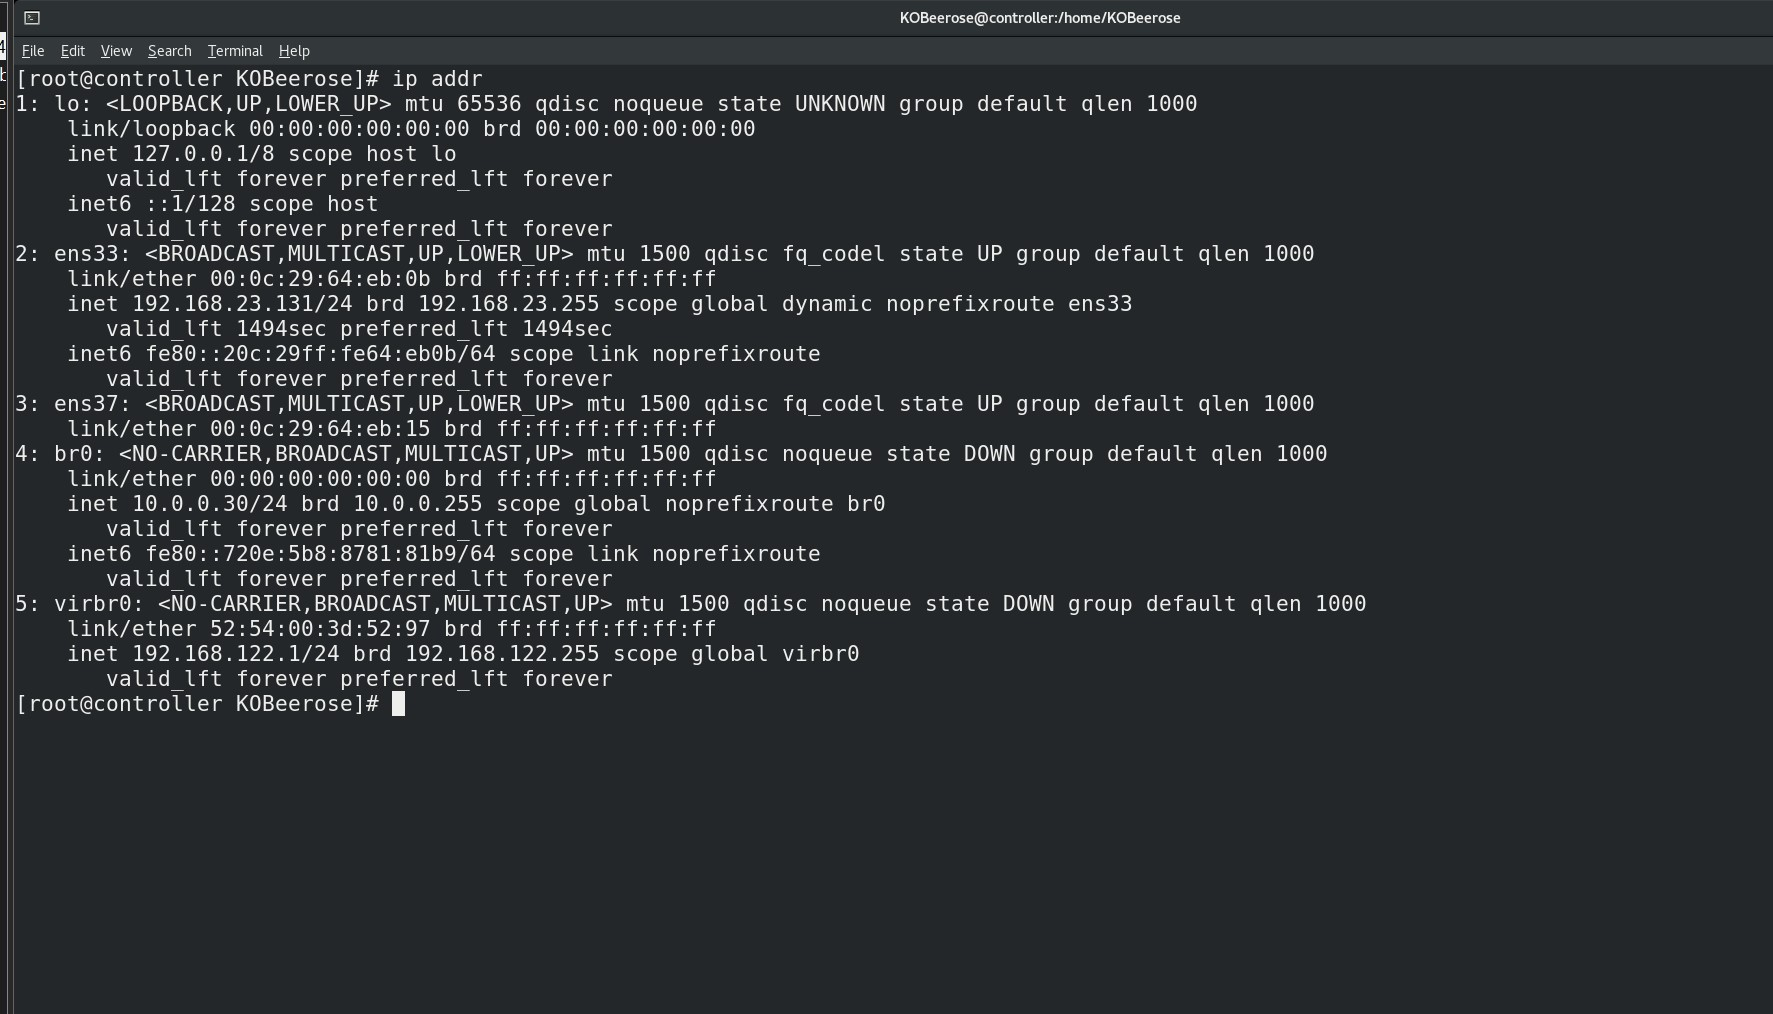
\includegraphics[width=1\linewidth]{Cloud/Add Virtual Machine Images/KVM Install/Checking network interfaces} 
\end{center} 
\caption{Checking network interfaces} 
\end{figure}  \FloatBarrier
\\

\section{KVM Install VM Management Tools}

\par we create an image of centos-8.0.\\

\\
\begin{figure}[!htb] 
\begin{center} 
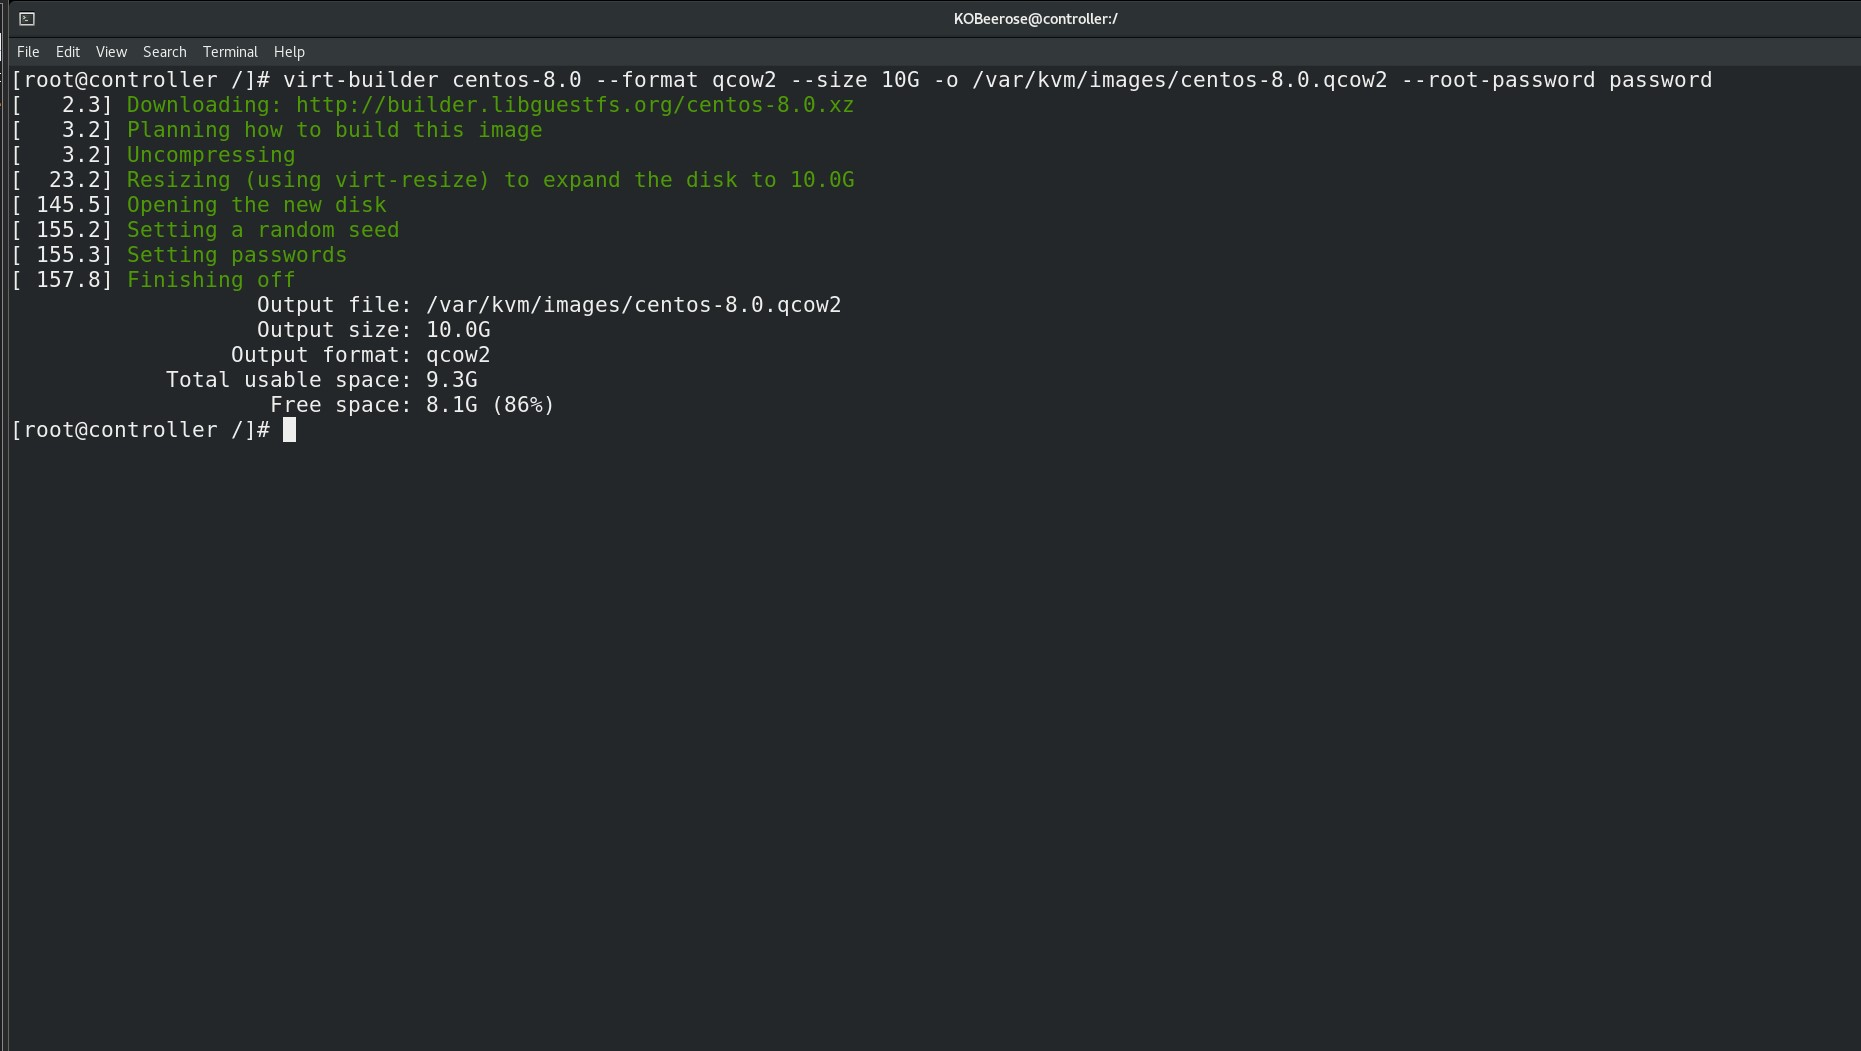
\includegraphics[width=1\linewidth]{Cloud/Add Virtual Machine Images/KVM Install VM Management Tools/creating a centos-8.0 IMG} 
\end{center} 
\caption{creating a centos-8.0 IMG} 
\end{figure}  \FloatBarrier
\\

\par to create a VM with the image above, we run the command virt-install
\\
\begin{figure}[!htb] 
\begin{center} 
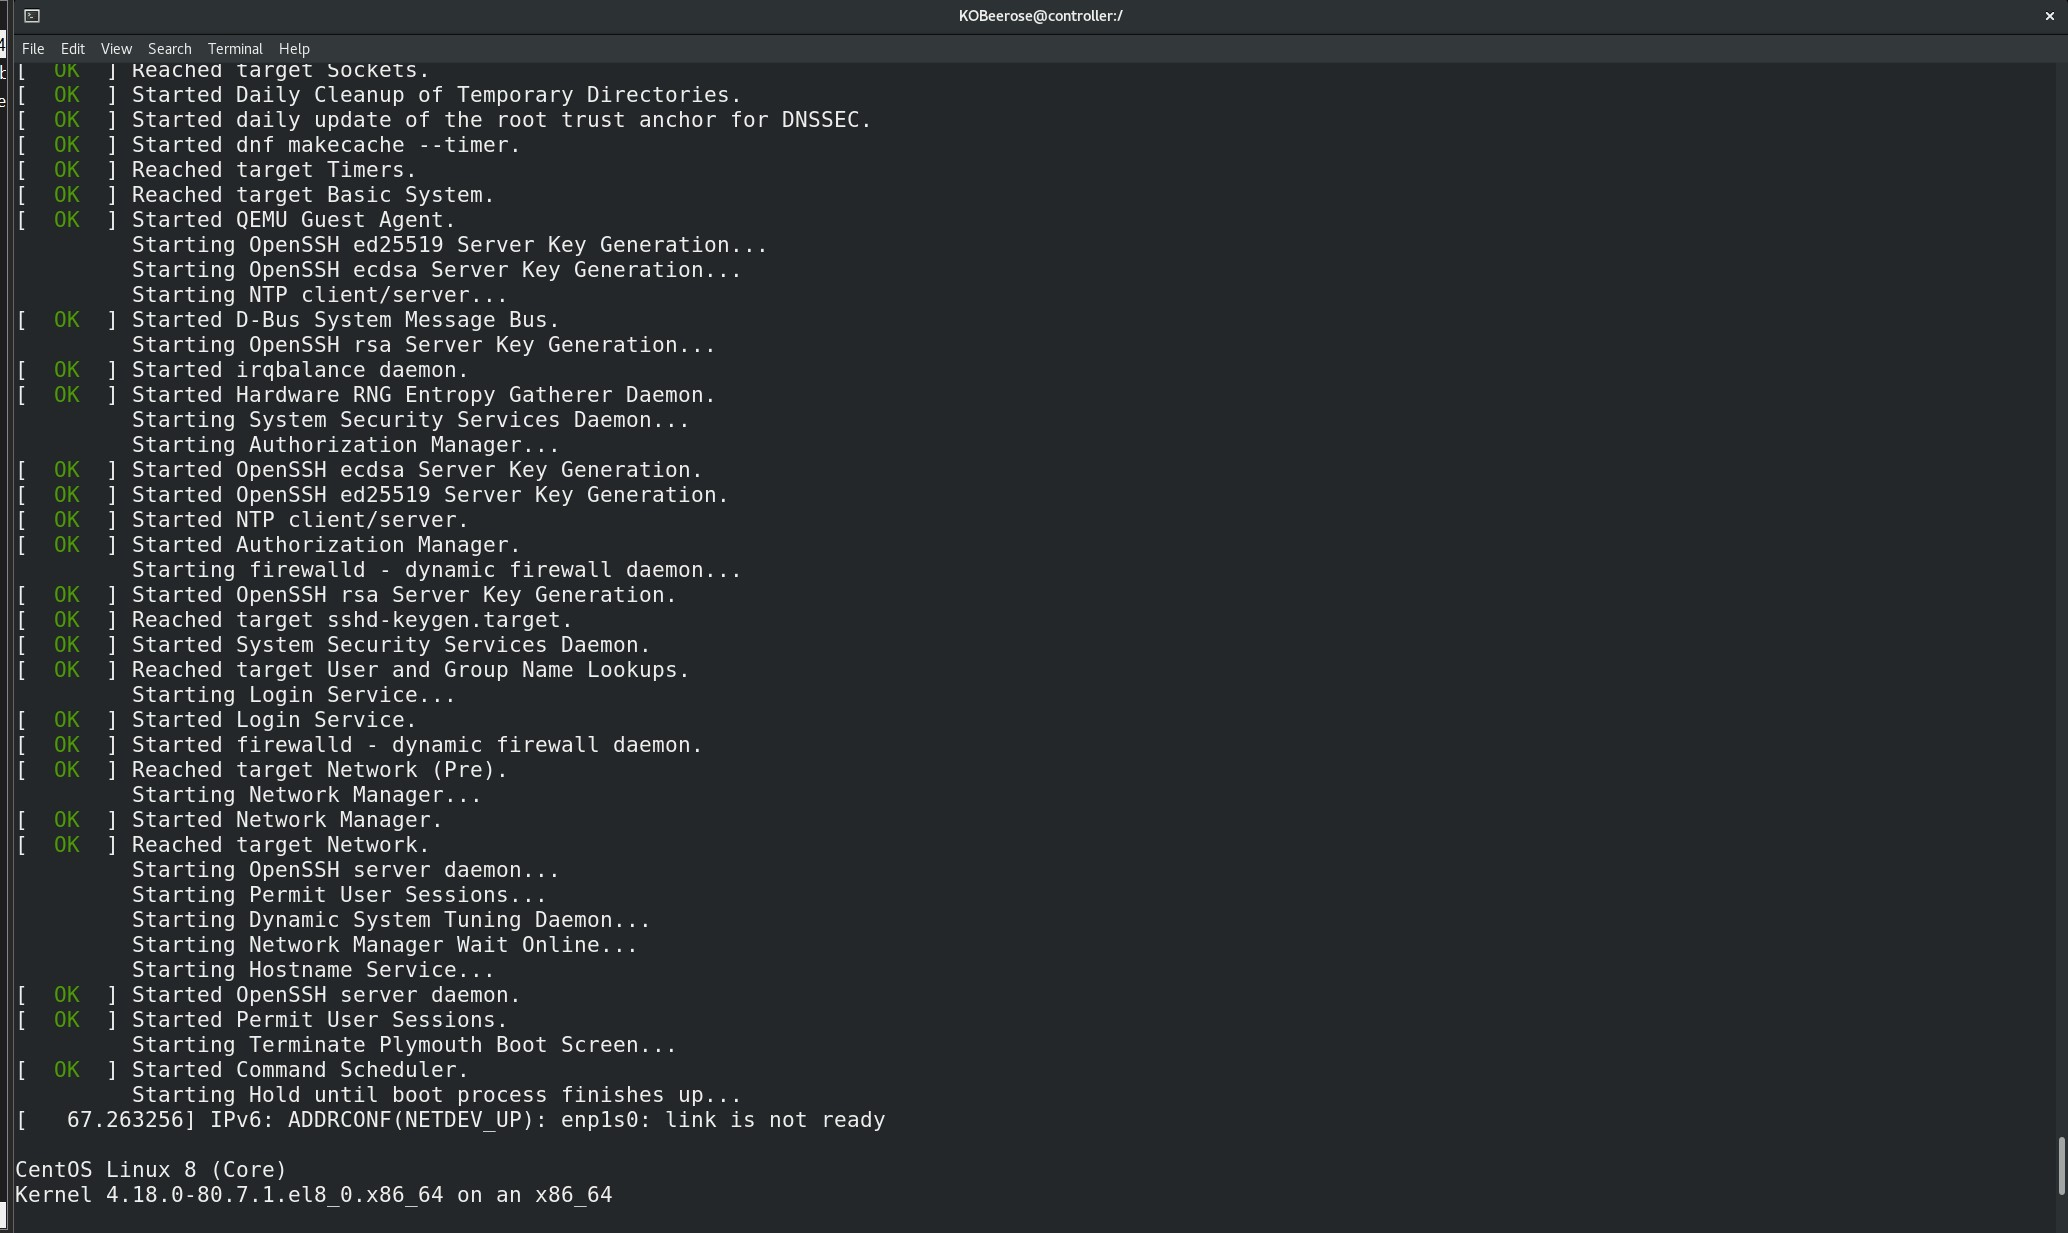
\includegraphics[width=1\linewidth]{Cloud/Add Virtual Machine Images/KVM Install VM Management Tools/Creating a VM with IMG} 
\end{center} 
\caption{Creating a VM with IMG} 
\end{figure}  \FloatBarrier
\\

\par 
Showing the content of a directory in a virtual machine.
\\
\begin{figure}[!htb] 
\begin{center} 
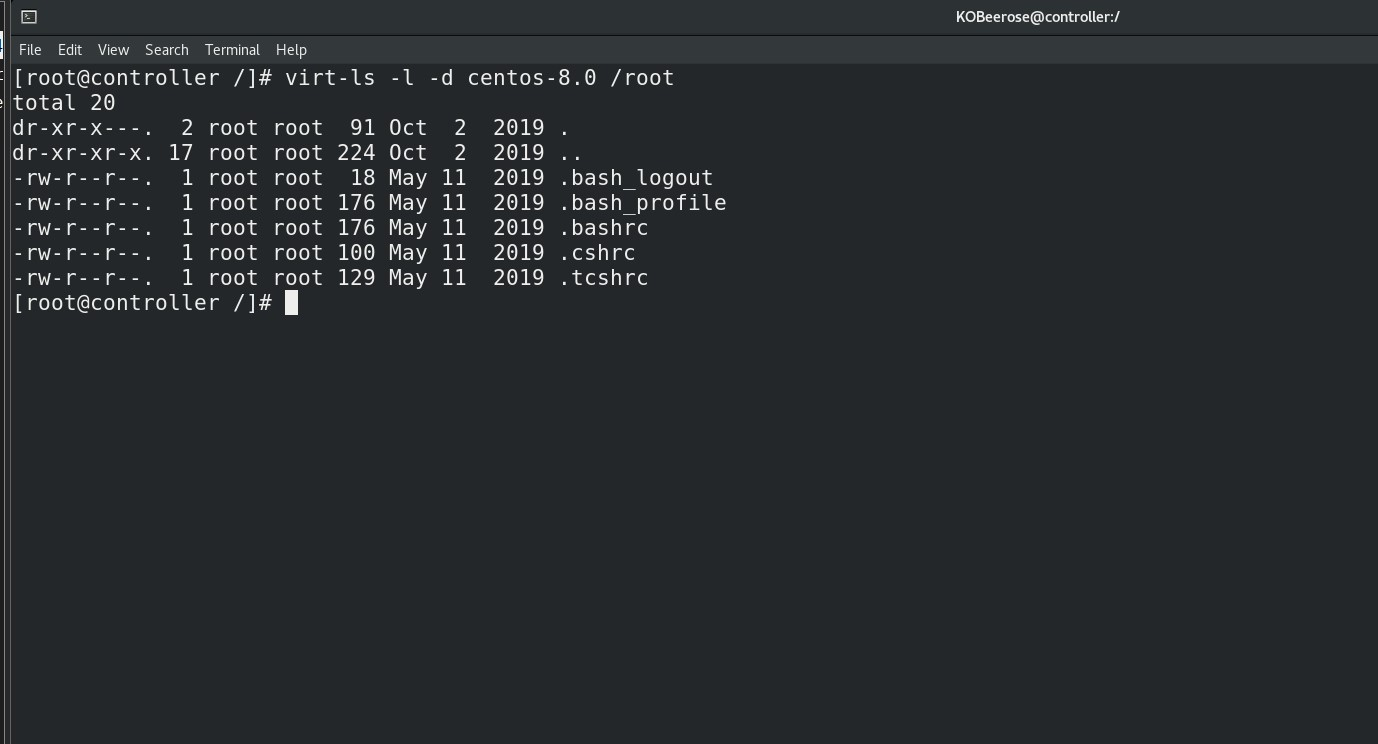
\includegraphics[width=1\linewidth]{Cloud/Add Virtual Machine Images/KVM Install VM Management Tools/VM dir check} 
\end{center} 
\caption{VM dir check} 
\end{figure}  \FloatBarrier
\\

\par 
Cat a file in a virtual machine, we will check the passwd file to be exact.
\\
\begin{figure}[!htb] 
\begin{center} 
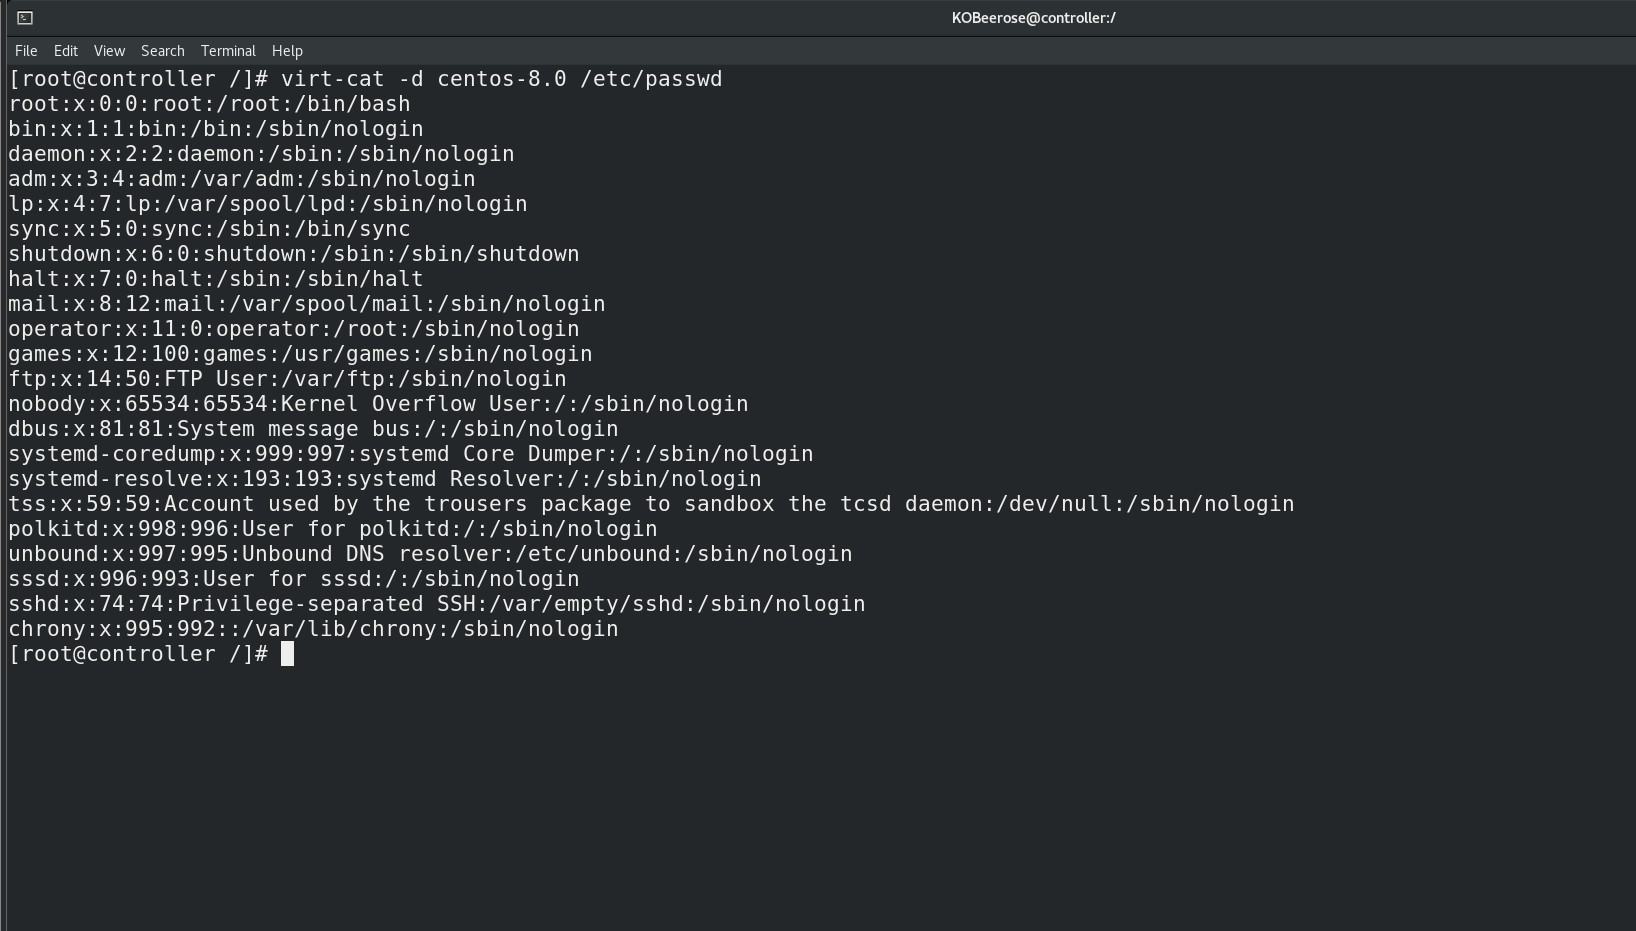
\includegraphics[width=1\linewidth]{Cloud/Add Virtual Machine Images/KVM Install VM Management Tools/Checking passwd file in VM} 
\end{center} 
\caption{Checking passwd file in VM} 
\end{figure}  \FloatBarrier
\\

\par 
now we Mount a disk for a virtual machine.
\\
\begin{figure}[!htb] 
\begin{center} 
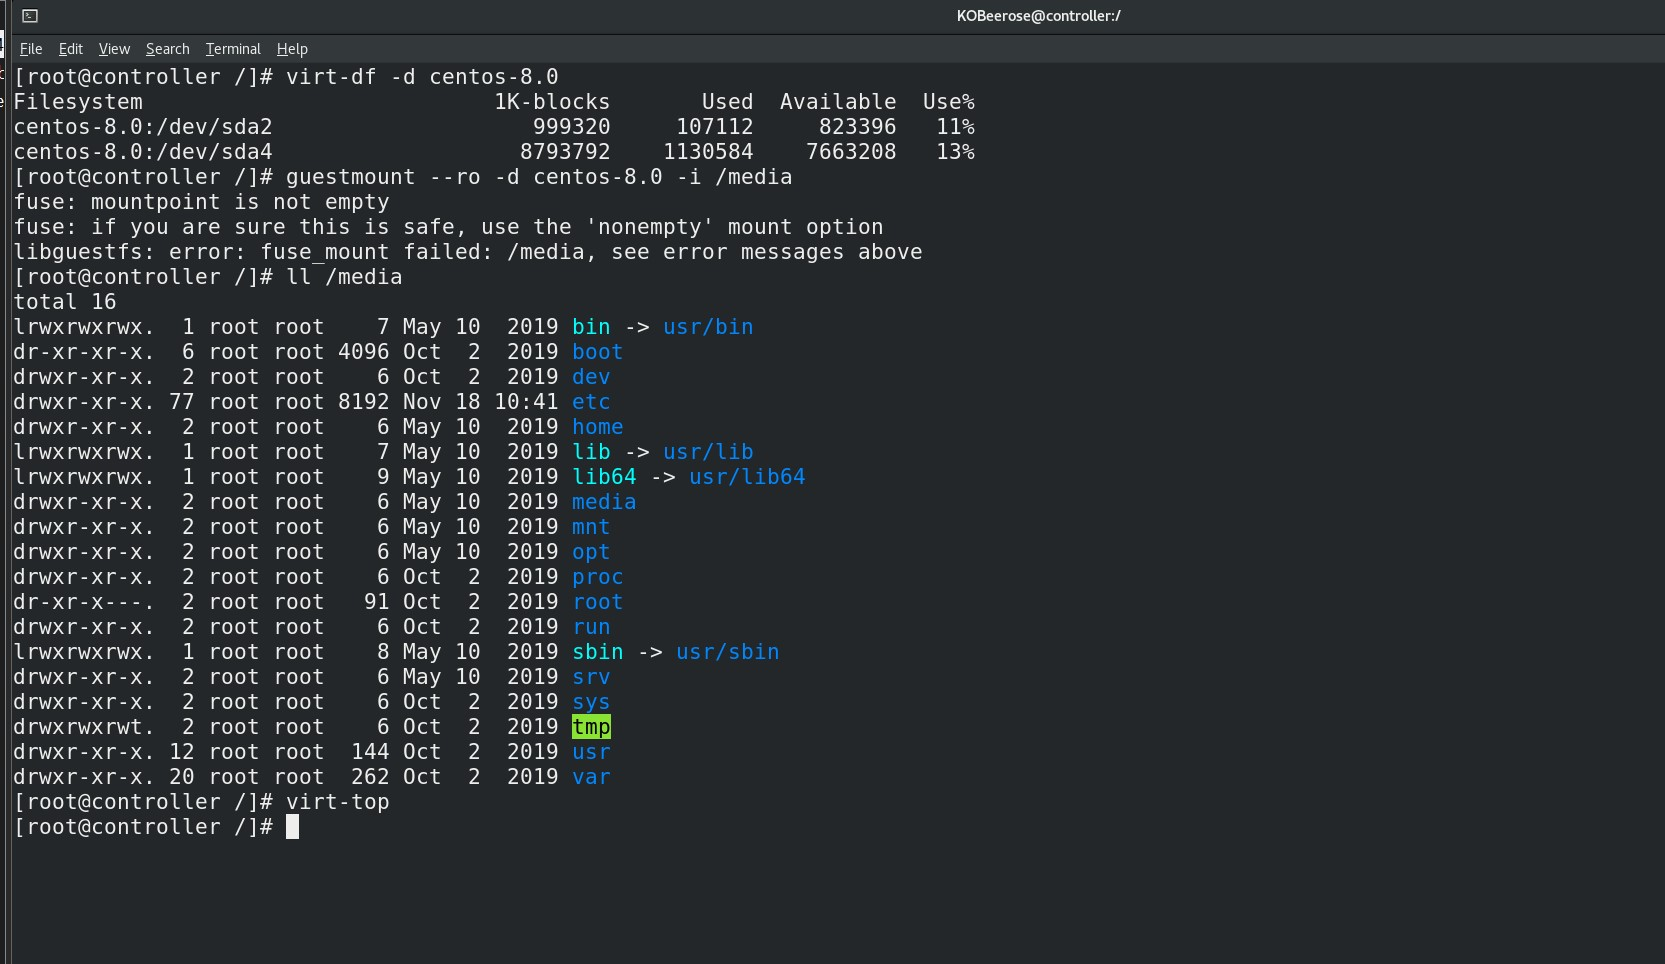
\includegraphics[width=1\linewidth]{Cloud/Add Virtual Machine Images/KVM Install VM Management Tools/Mount a disk for VM} 
\end{center} 
\caption{Mount a disk for VM} 
\end{figure}  \FloatBarrier
\\

\section{Add VM Images}

\par To create a CentOS 8 image on the Glance service host. we will first create a folder that will contain the disk image, then download the official centos-8.2 image.


\begin{figure}[!htb] 
\begin{center} 
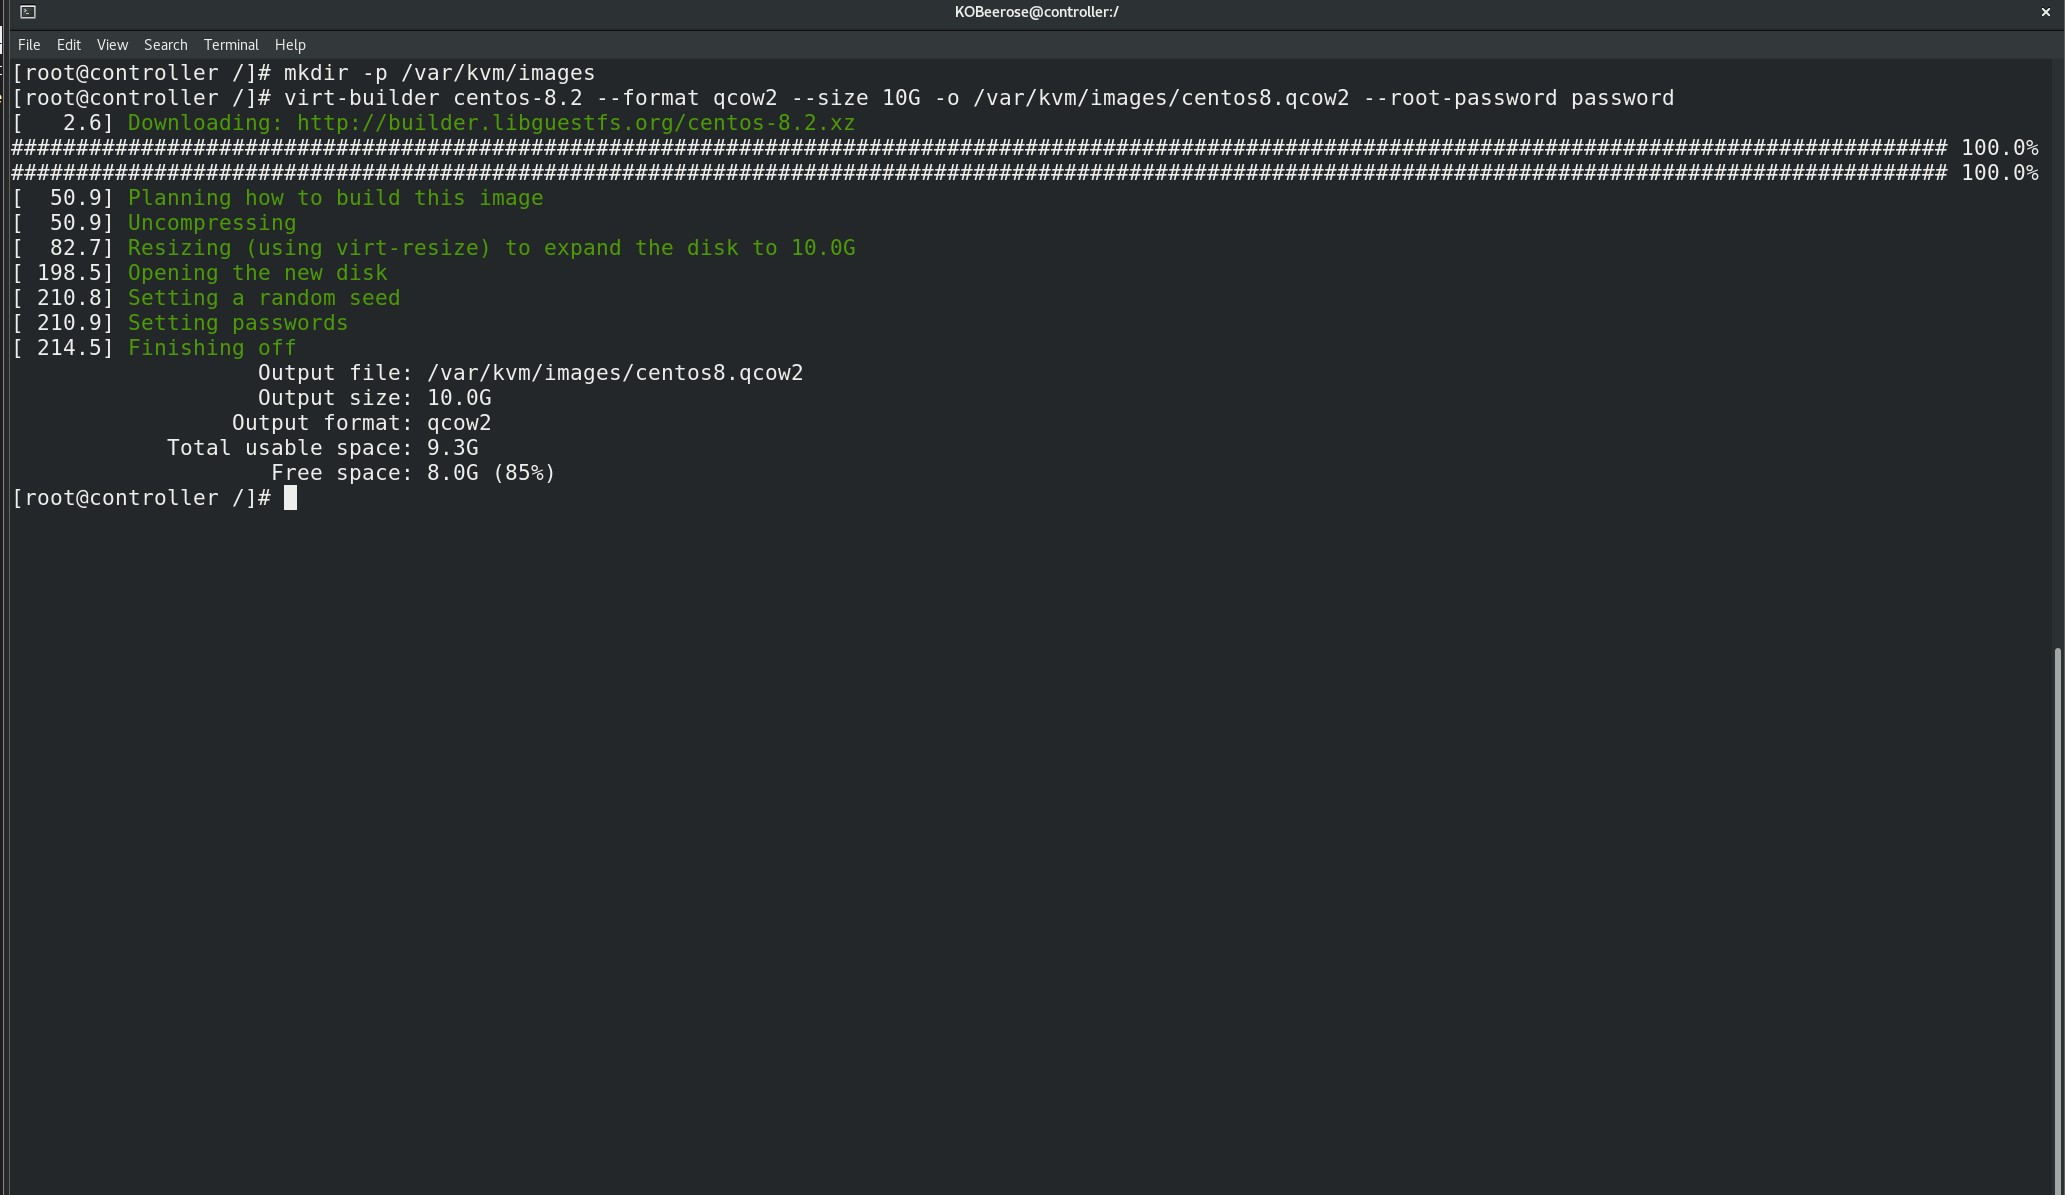
\includegraphics[width=0.93\linewidth]{Cloud/Add Virtual Machine Images/Add VM Images/Download official IMG} 
\end{center} 
\caption{Download official IMG} 
\end{figure}  \FloatBarrier

\par We will install the image loaded by virt-install and just after booting the VM, we will connect and configure some necessary parameters: 


\begin{figure}[!htb] 
\begin{center} 
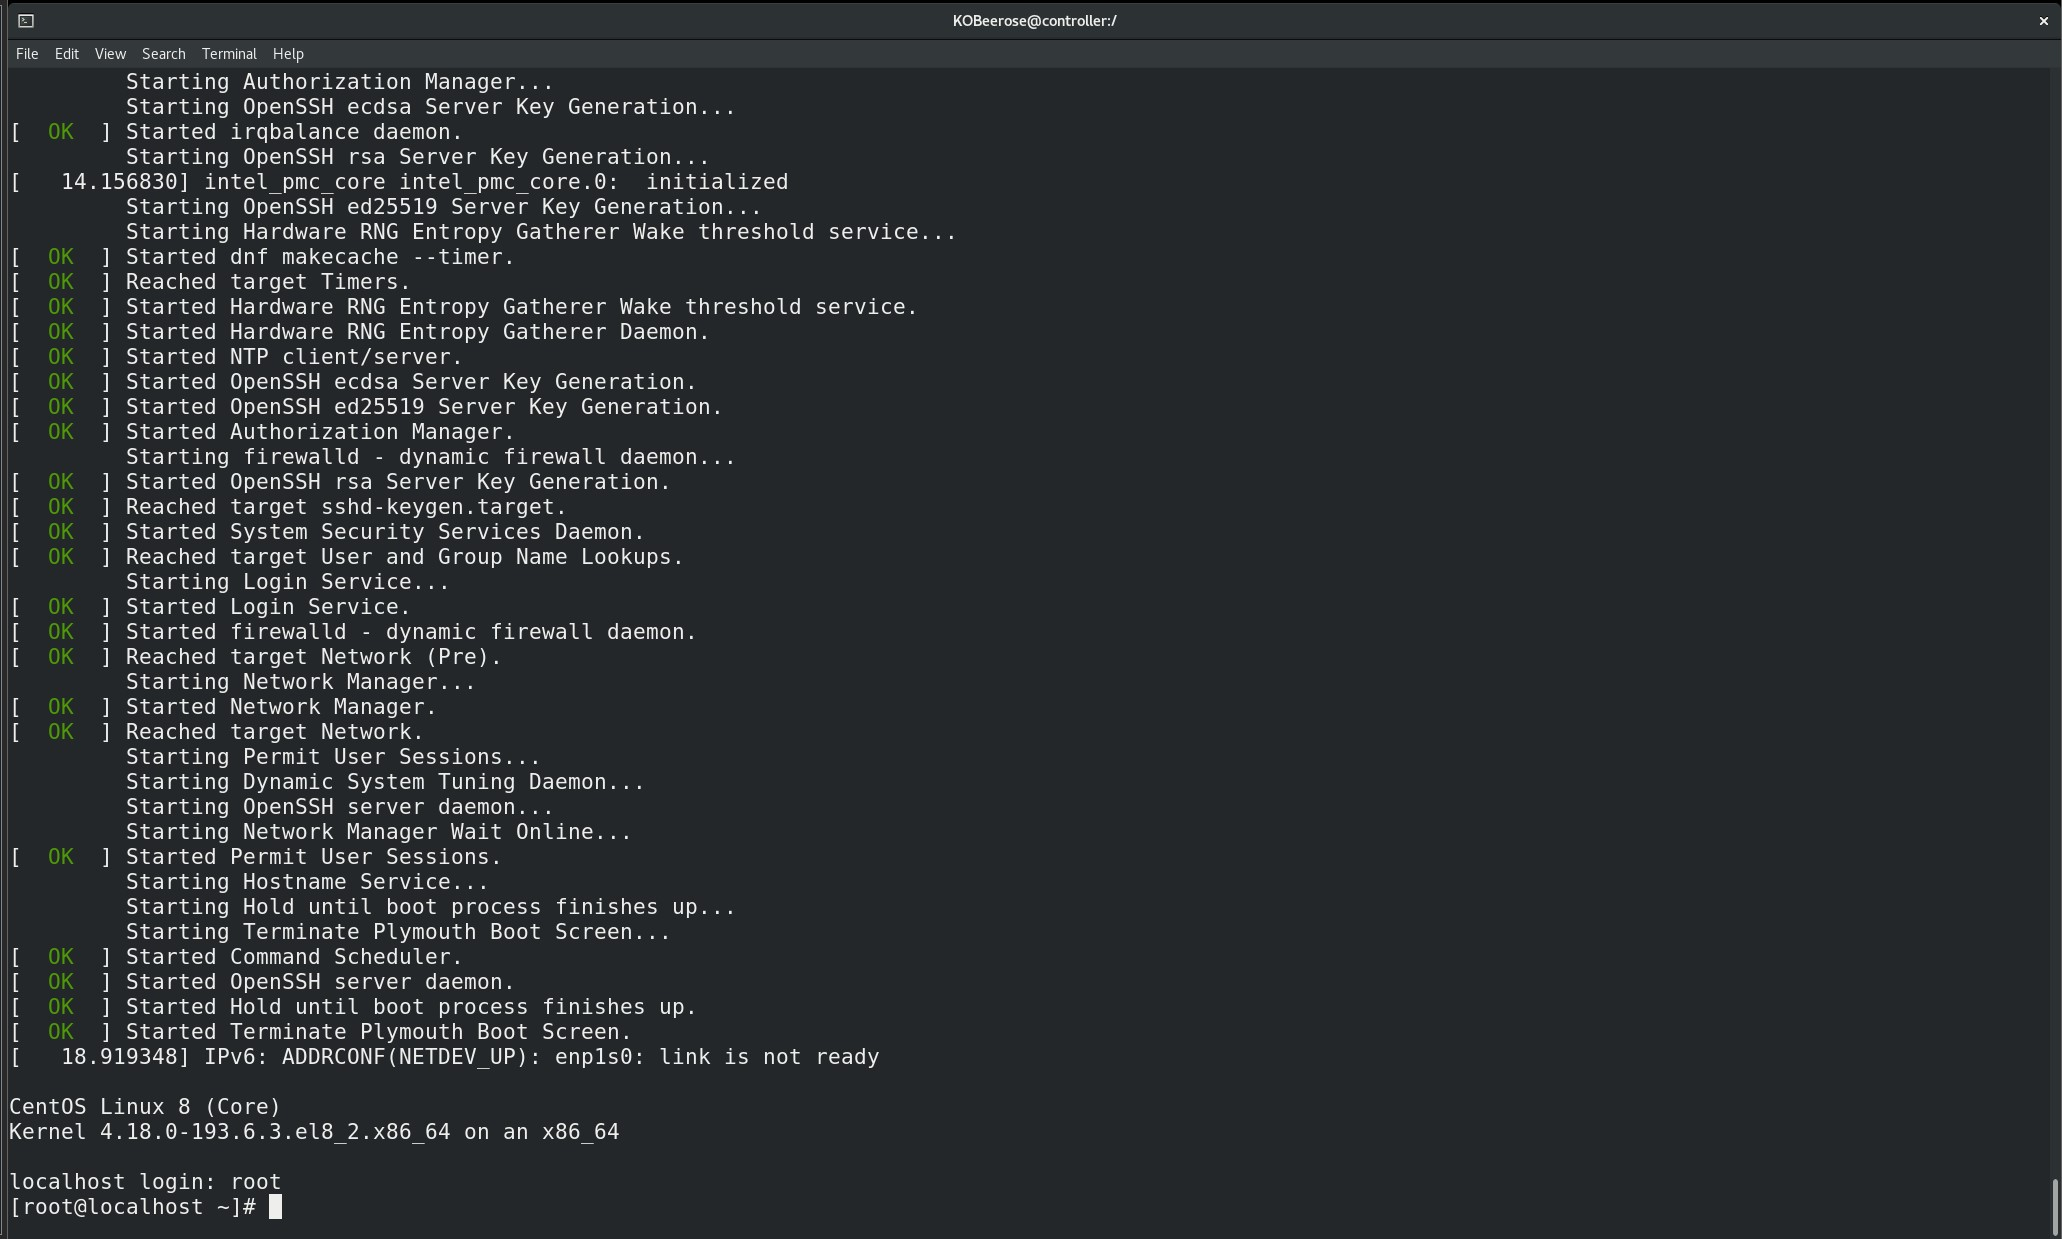
\includegraphics[width=0.93\linewidth]{Cloud/Add Virtual Machine Images/Add VM Images/Installing centos8.2 IMG} 
\end{center} 
\caption{Installing centos8.2 IMG} 
\end{figure}  \FloatBarrier
\\
\par Now that our Virtual Machine is installed we login and configure some necessary settings.

\\
\begin{figure}[!htb] 
\begin{center} 
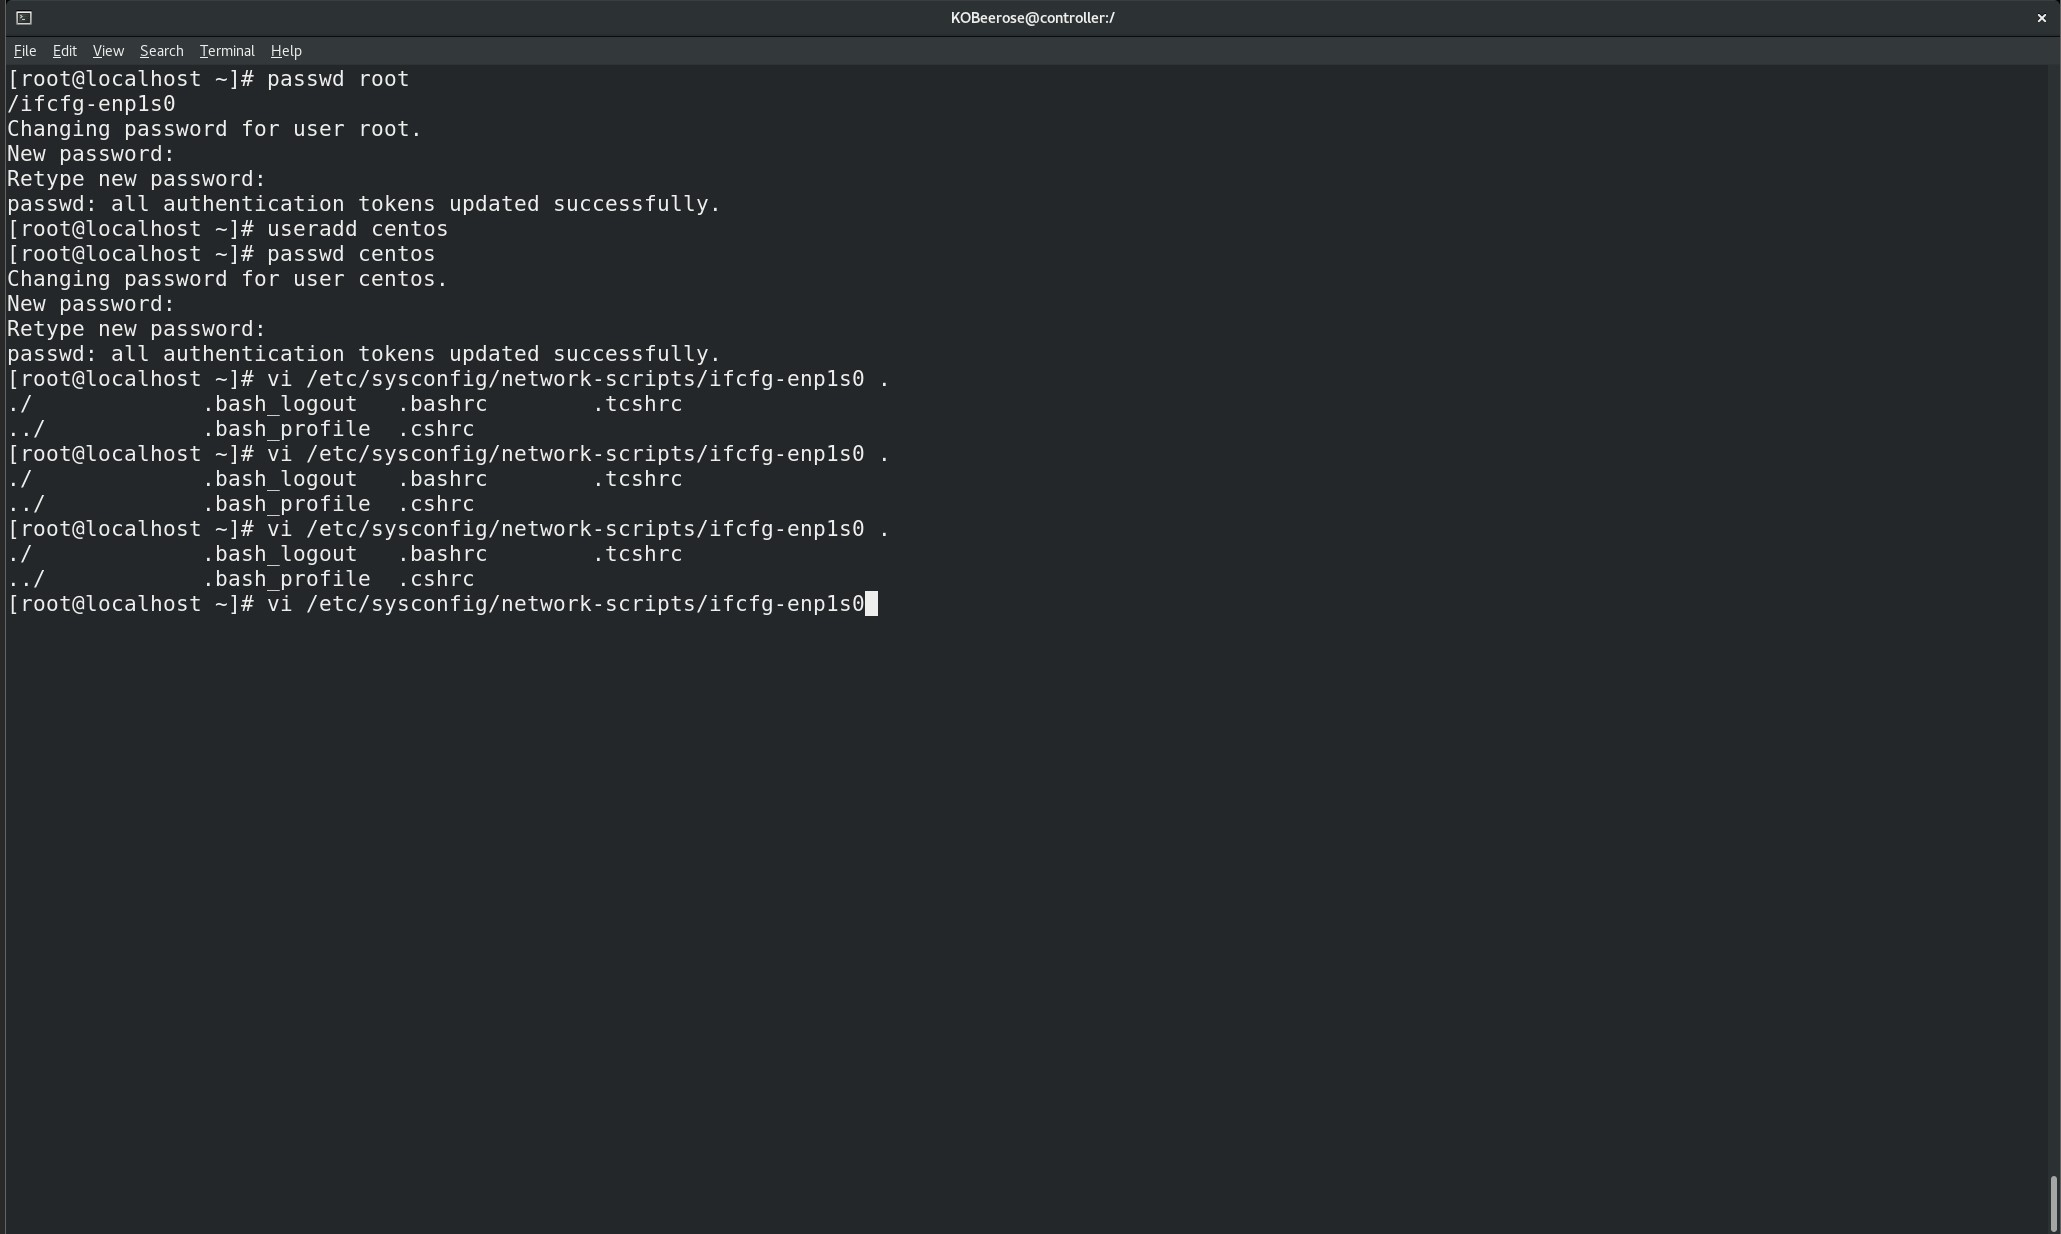
\includegraphics[width=1\linewidth]{Cloud/Add Virtual Machine Images/Add VM Images/Manage Users} 
\end{center} 
\caption{Manage Users} 
\end{figure}  \FloatBarrier
\\


\par After that, we will install cloud-init and openssh-server. 
\\
\begin{figure}[!htb] 
\begin{center} 
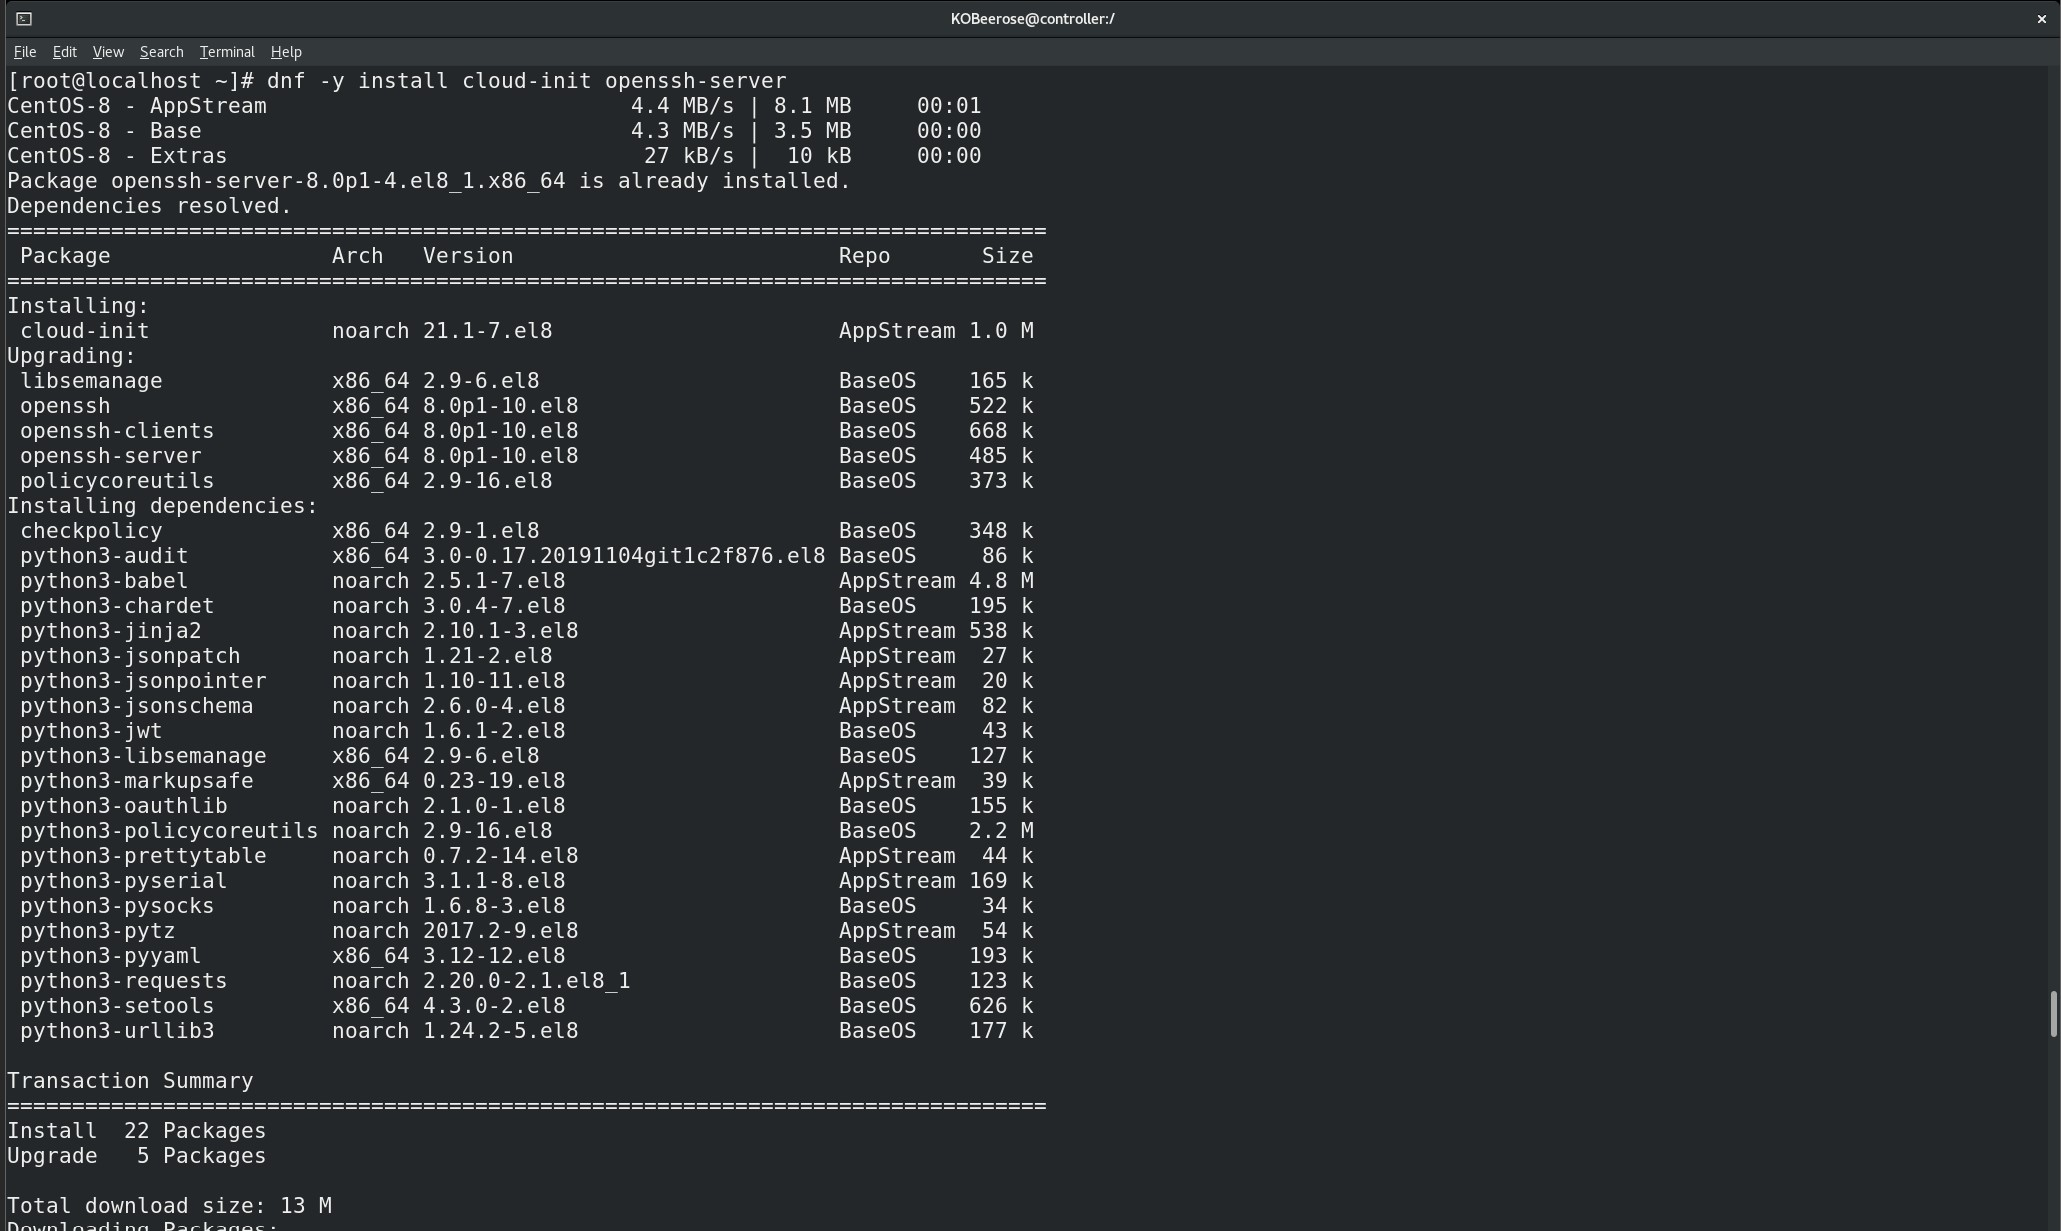
\includegraphics[width=1\linewidth]{Cloud/Add Virtual Machine Images/Add VM Images/Installing cloud-init} 
\end{center} 
\caption{Installing cloud-init} 
\end{figure}  \FloatBarrier
\\

\par We are going to modify the cloud configuration by modifying the file /etc/cloud/cloud.cfg,
by authorizing password authentication via SSH and changing to [centos] as user
by default. We will then activate cloud-init sshd and shut down the VM. 
\\
\begin{figure}[!htb] 
\begin{center} 
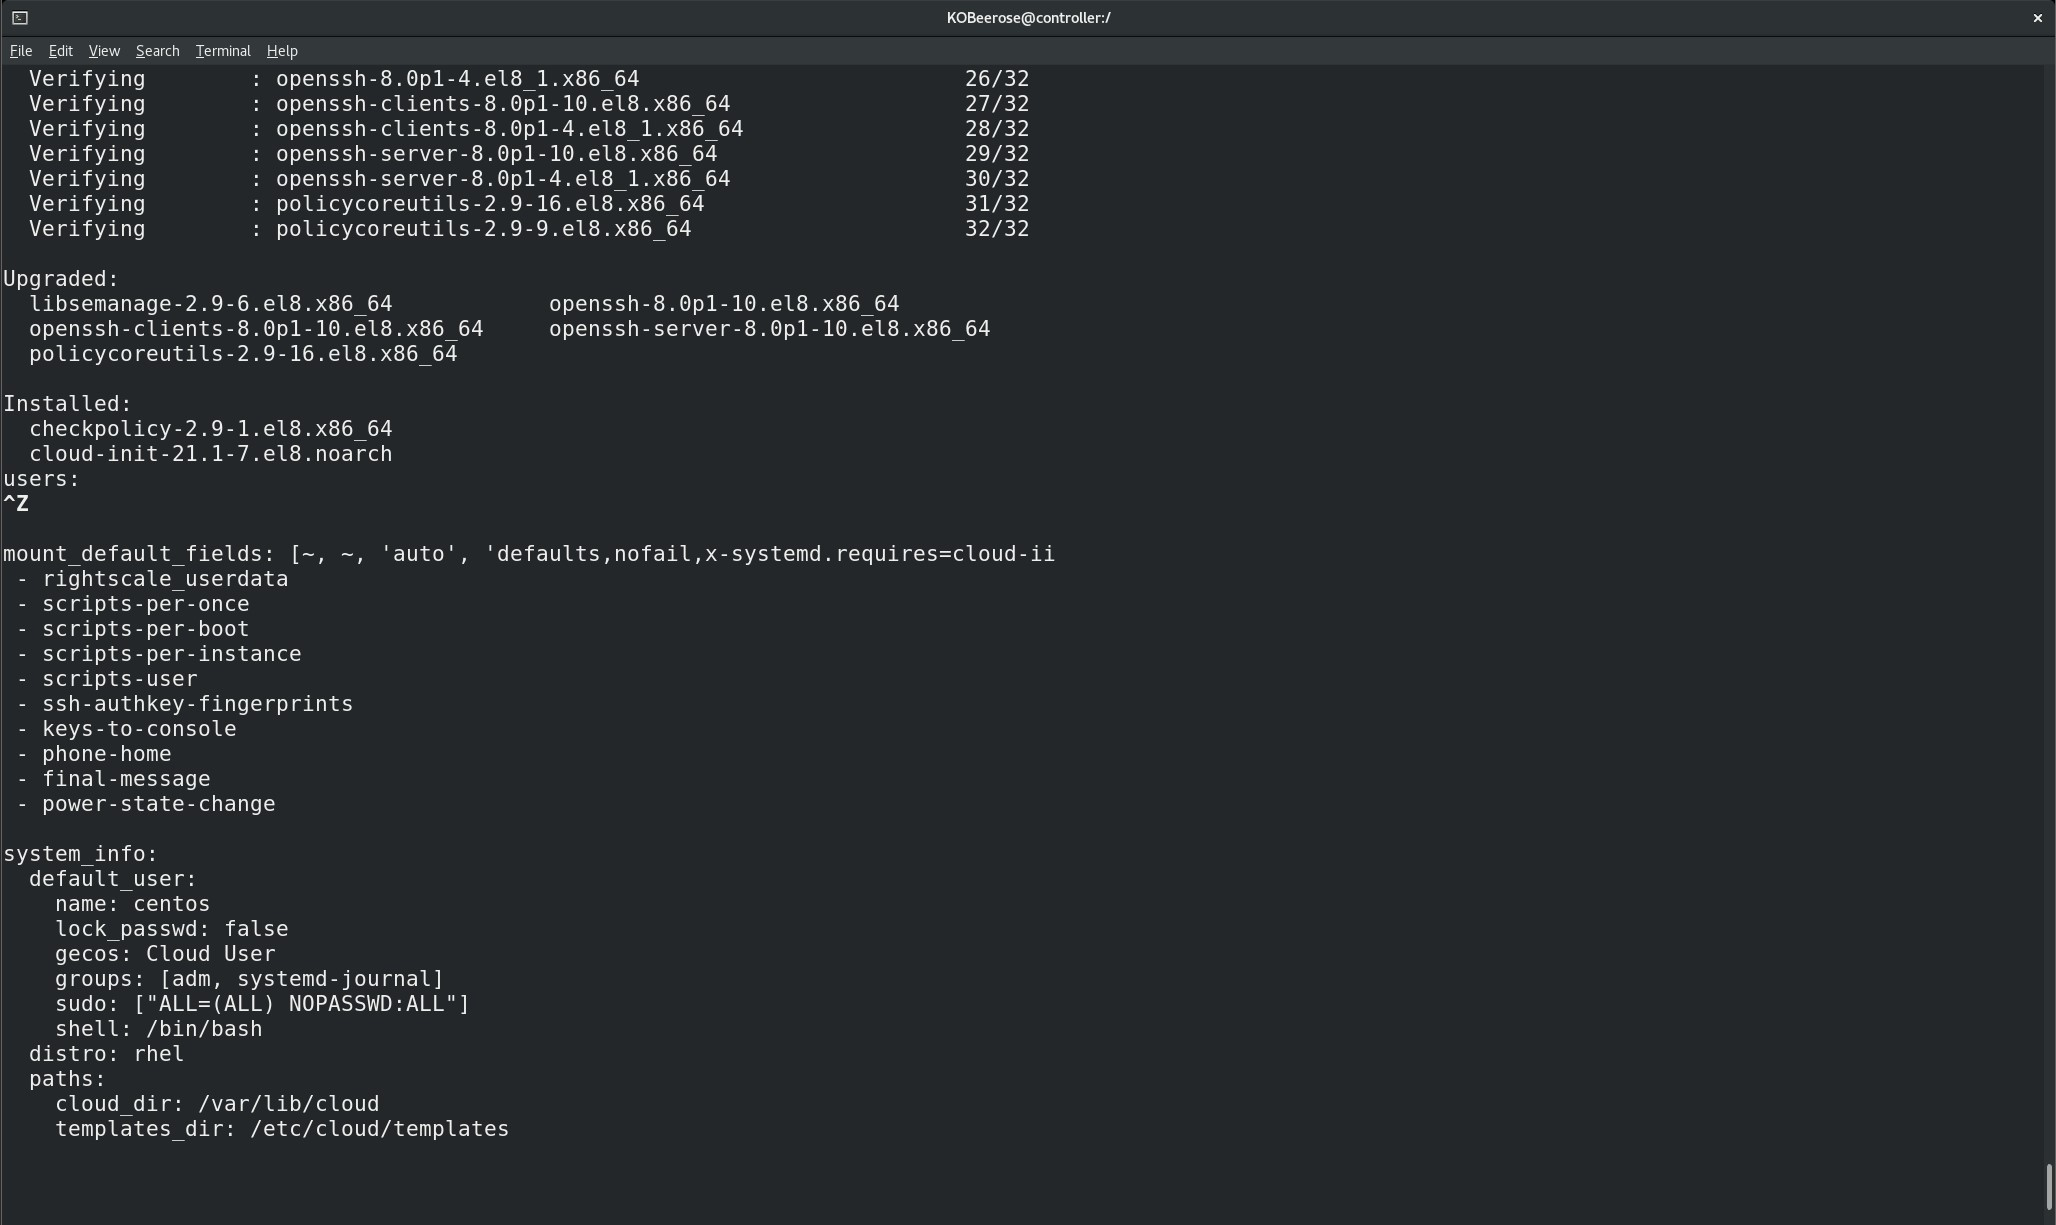
\includegraphics[width=1\linewidth]{Cloud/Add Virtual Machine Images/Add VM Images/Editing cloud.cfg file} 
\end{center} 
\caption{Editing cloud.cfg file} 
\end{figure}  \FloatBarrier
\\

\par we should enable the cloud-init sshd.
\\
\begin{figure}[!htb] 
\begin{center} 
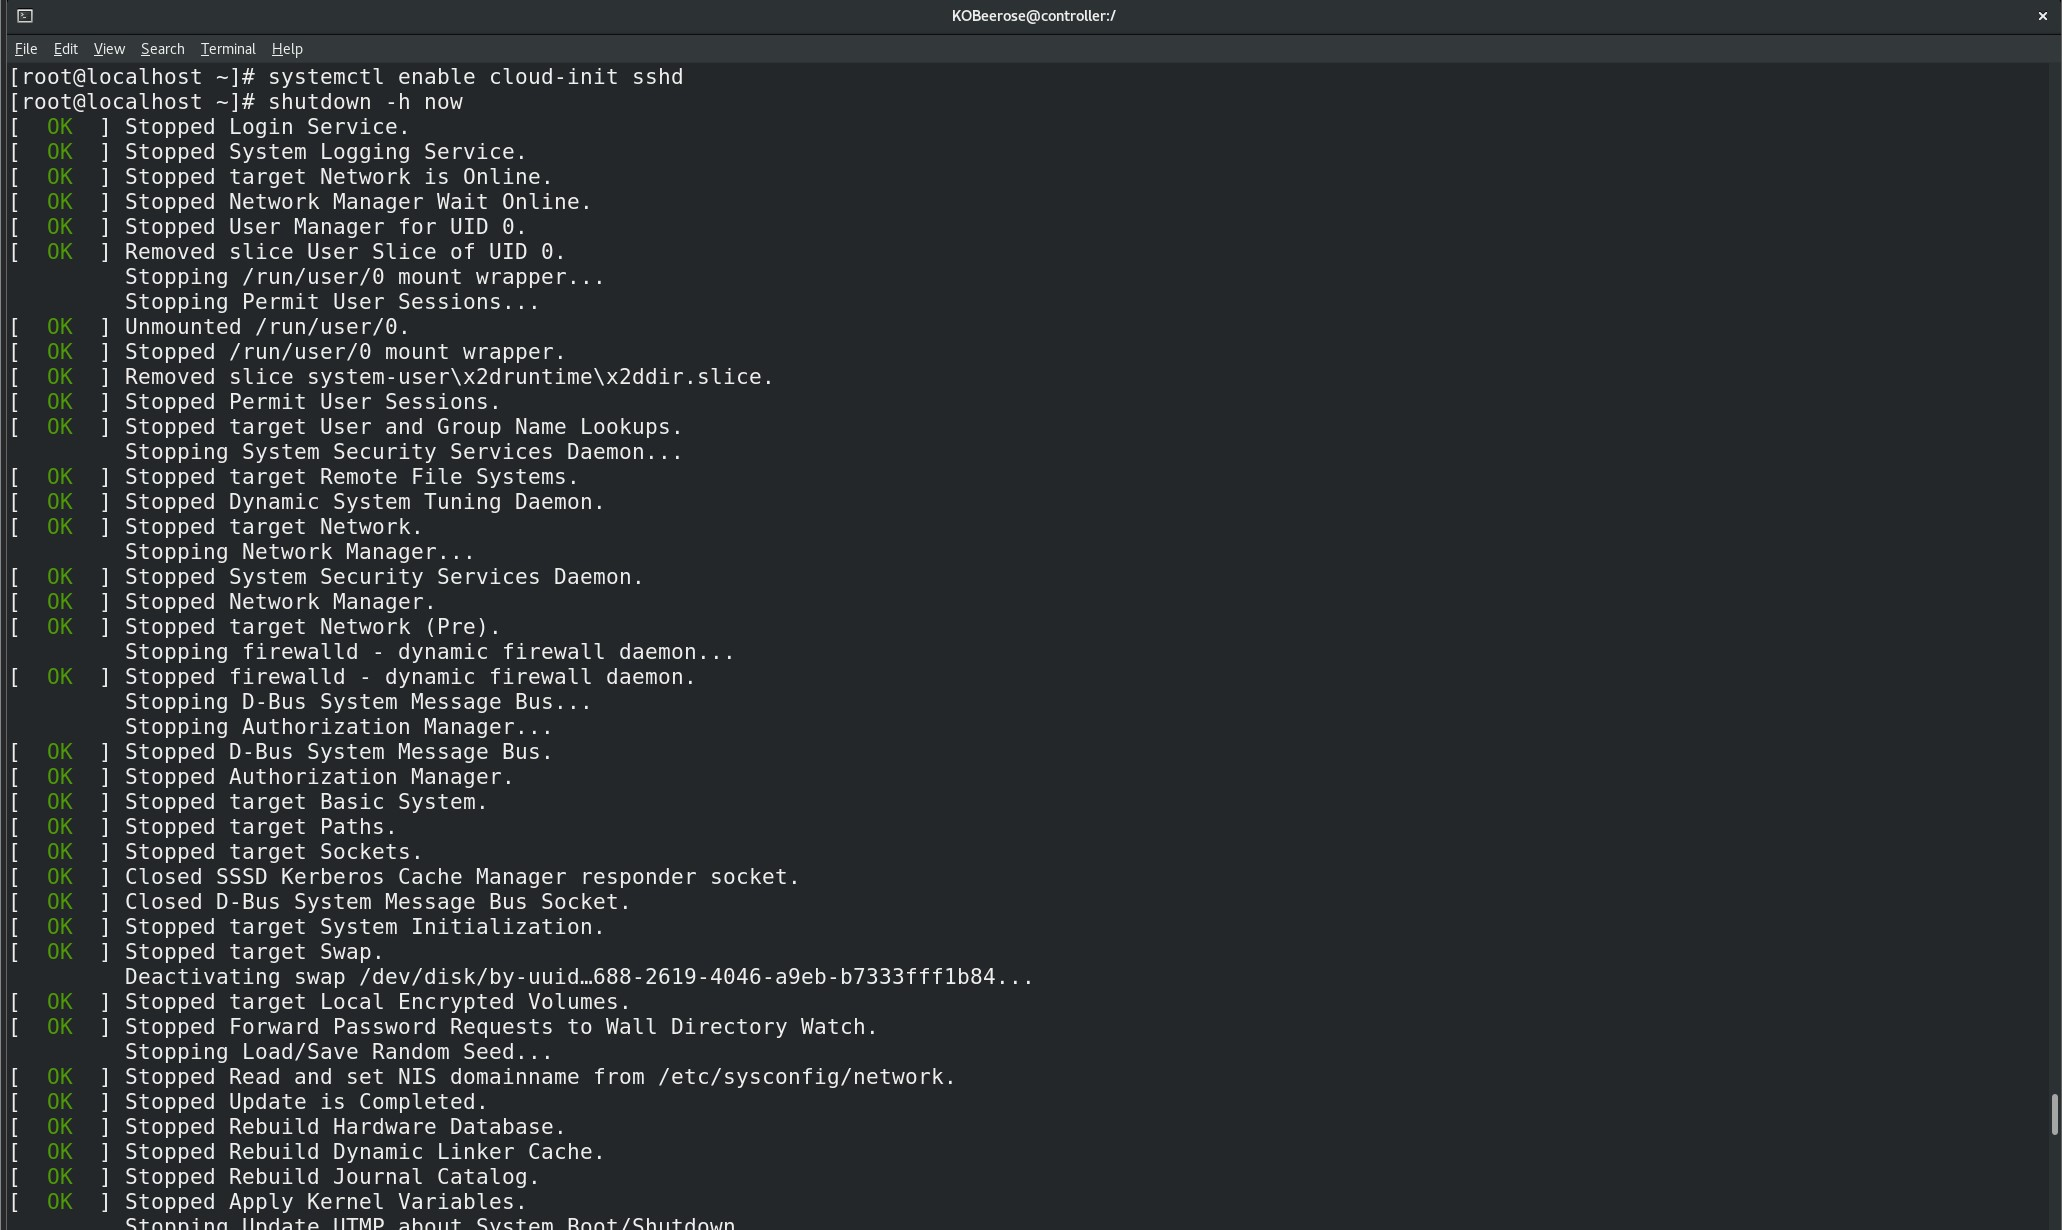
\includegraphics[width=1\linewidth]{Cloud/Add Virtual Machine Images/Add VM Images/Enabling cloud-intit} 
\end{center} 
\caption{Enabling cloud-intit} 
\end{figure}  \FloatBarrier
\\

\par After adding a virtual image to Glance, we can display the whole list of images. 

\\
\begin{figure}[!htb] 
\begin{center} 
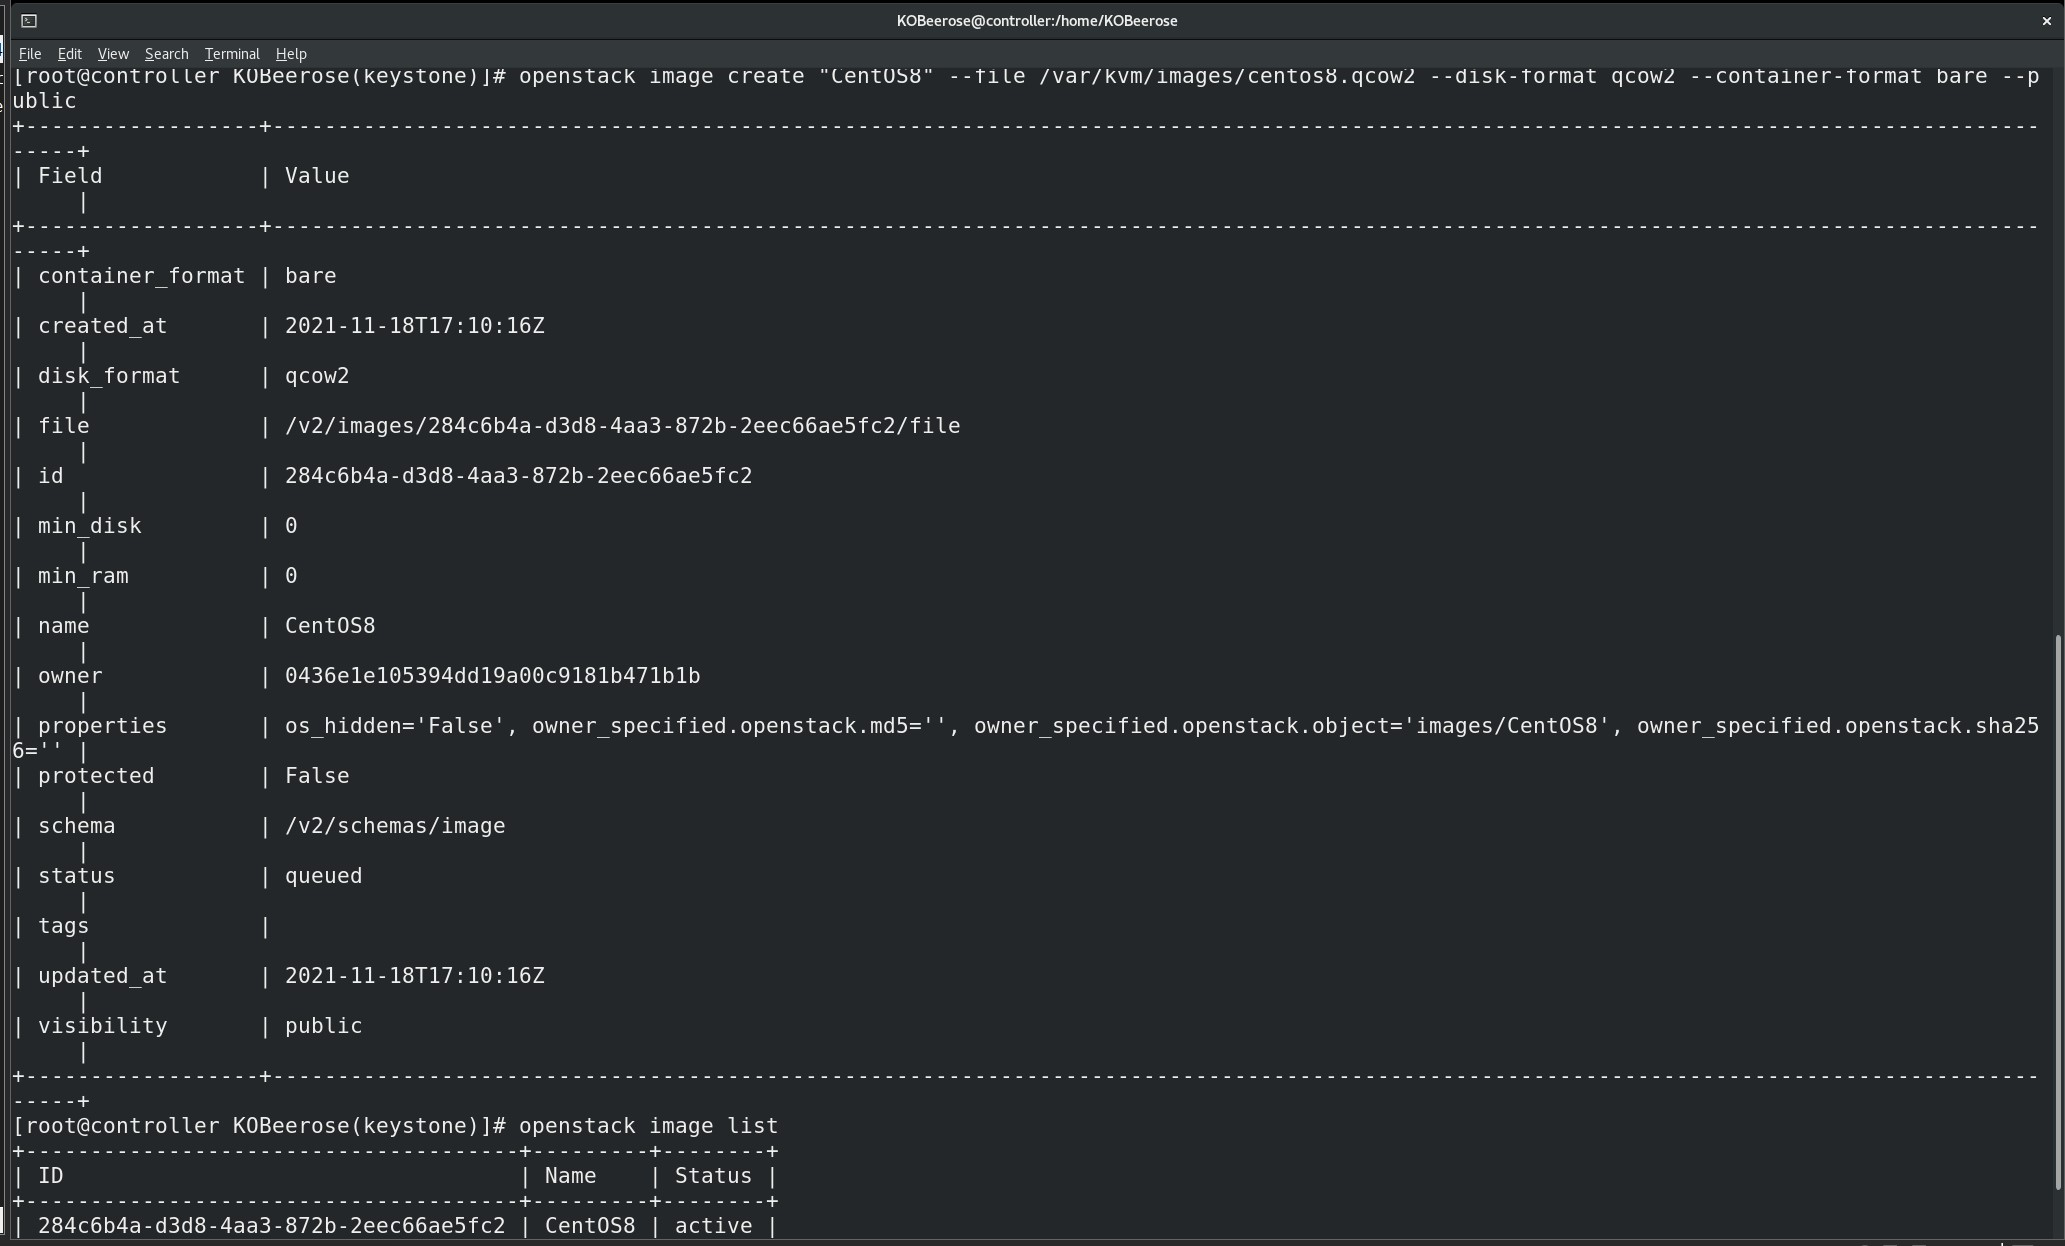
\includegraphics[width=1\linewidth]{Cloud/Add Virtual Machine Images/Add VM Images/Add VM to Glance} 
\end{center} 
\caption{Add VM to Glance} 
\end{figure}  \FloatBarrier
\\
\end{spacing}